%BEGIN JC
\subsection{Isosurface Contouring}
Now when the optimized voxel data was obtained, the next step is to generate a \emph{mesh based
geometry}. It will be useful in the further NURBS implementation. In order to achieve it, the
data will be represented by a contour of a smooth function, rendering an isosurface. The
isosurface allows to visualize Scalar Volumetric Data in 3D. It furthermore permits a mesh
representation of the volume data. The mesh can be composed of triangles or quads, according
to the algorithm used. There are two main approaches to solve this problem, the most
famous one is Marching Cubes.

\begin{figure}
\centering
   \scalebox{0.8}{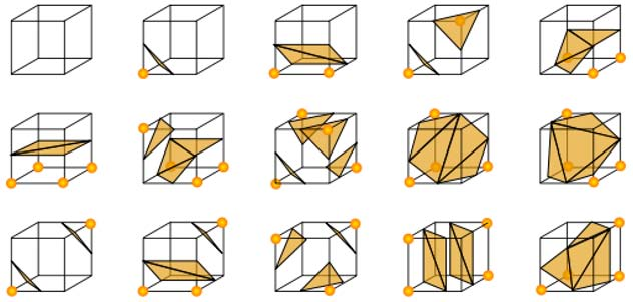
\includegraphics{Pictures/cubes.pdf}}\\
   \caption{Basis cases of Marching Cubes}
\end{figure}

\subsubsection{Marching Cubes} 

This algorithm takes as an input a regular volumetric data set and extracts a polygonal mesh. It
divides the space into cubes, which are defined by the volume information. Each cube has scalar
information on its vertices, the value is equal or above a marked isovalue. Therefore each of the
eight vertices of a cube can be marked or unmarked. According to these values vertices are drawn
on the edges of the cube at calculated points with the use of interpolation. A cube that contains
an edge is called active. Non active cubes are not further considered in the algorithm.

By connecting the vertices we obtain a polygon on each cube. There are 256 possible scenarios,
but most of them are just reflections or rotationally symmetric cases of each other. Therefore
there are 15 base cases which represent all the possibilities of the marching cubes (Figure 2.1). 
The original algorithm presents two main problems. Firstly it does not guarantee neither
correctness nor topological consistency, which means that holes may appear on the surface due
to inaccurate base case selection. The second problem is ambiguity, which appears when two
base cases are possible and the algorithm chooses the incorrect one. These cases can be grouped
into face ambiguities and internal ambiguities. There are many extended Marching Cubes
algorithms that tackle the problems of the original one, getting rid of the ambiguities and
providing correctness.

\subsubsection{Dual Contouring}
The idea of this algorithm is similar to Marching Cubes, but instead of generating vertices on the
edges of the cubes, it locates them inside the cube. Figure 2.5 shows the basic differences in both approaches.
The vertices associated with the four contigous cubes are joined and form a quad. The question now is
which place inside the cube is the ideal one to insert each vertex. Different dual algorithms are classified 
according to the answer for this question. Dual contouring generates a vertex positioned at the minimizer of a
quadratic function which depends on the intersection points and normals. Therefore the method needs Hermite 
data to work with.
\begin{equation*}
E(x)= x^TA^TAx-2x^TA^Tb+b^Tb
\end{equation*}
Where \textit{A} is a matrix whose rows are the normals and \textit{b} is a vector whose entries are the product of normals and intersection points. To solve this system, a nummerical treatement is needed. As proposed in [1] the best approach is to compute the
SVD decomposition of \textit{A} and form the pseudo-inverse by truncating its small singular values. 
%1=Dual Contouring of HErmite DAta


The main advantage of this method over MC is the adquisition of better aspect ratios. On the other hand the need of Hermite Data
represents a disadvantage. Furthermore there is no open source algorithm that implements the Dual Contouring scheme.


\subsection{The VTK Toolbox}
\subsubsection{Installing VTK}
VTK was installed using the Linux platform, for it to be successfully implemented a gcc compiler
must be already on the machine. VTK offers the possibility to use Python, TLC or C++ for
development. VTK toolbox is actually a C++ library, which is implemented in other languages. We
decided to continue the project with C++ since it gives the possibility to explore the original code.
A few dependency problems were encountered, nevertheless they were easy to track back. If any
problems were to be found at installation time, please refer to the VTK Wiki where the procedure
is explained step by step.

\begin{figure}
\centering
   \scalebox{0.35}{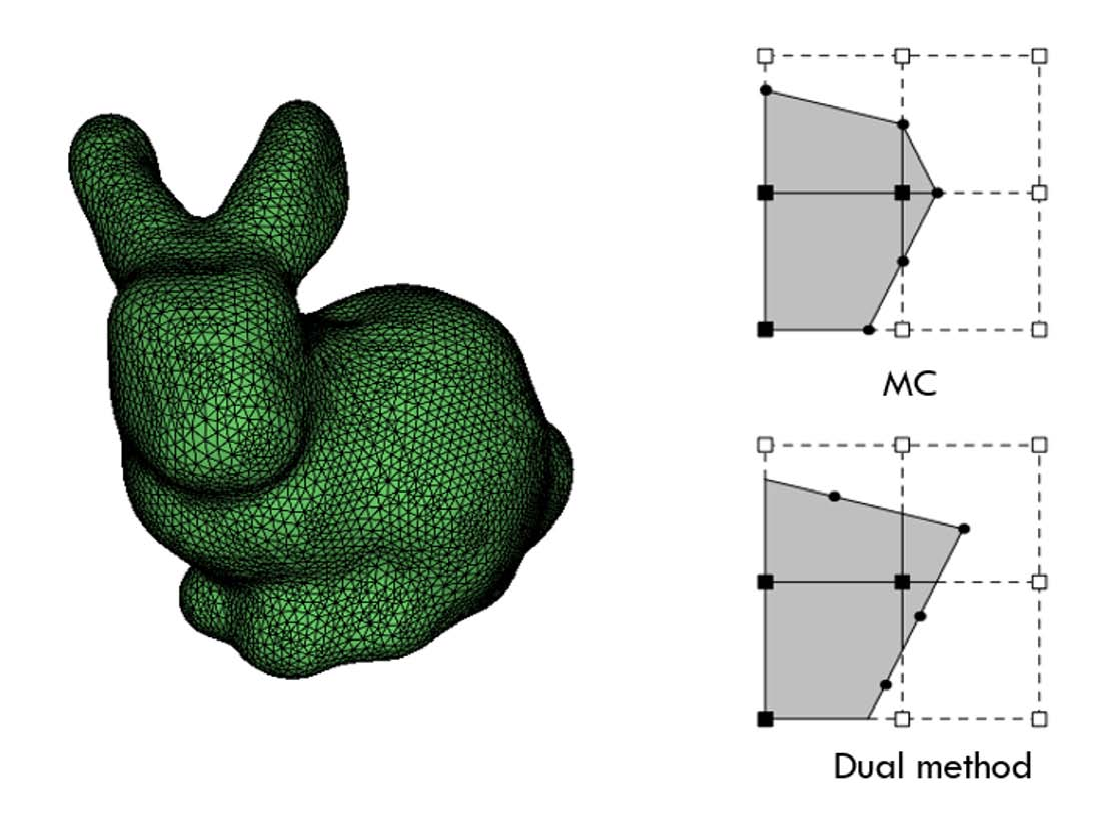
\includegraphics{Pictures/bunny_MC.pdf}}\\
   \caption{\textit{Right:} The famous Standford Bunny. \textit{Left:} Main difference between MC and Dual methods }
\end{figure}

\subsubsection{Implementing the VTK Classes}
The VTK toolbox was used in order to implement the algorithms on our optimized data. It is a heavily object
oriented toolbox. Our first approach was to use the built in Marching Cubes algorithm,
nevertheless it did not work with our unstructured grid data. It just works for ImageData and
PolyData . For structured and unstructured grids the tool to render the isosurface is the contour
Filter tool. Unfortunately the documentation does not present which algorithm the tool uses. It
can be inferred that it is an extended Marching cube algorithm.

The Contour Filtering seemed to work fine but the visualization of our data was still not possible
and an intermediate step was needed. We used the Implicit Modelling tool which is a filter that
computes the distance from the input geometry to the points of an output structured point set.
This distance function can then be "contoured" to generate new, offset surfaces from the original
geometry. It finally allowed visualization but it created one problem. Holes are lost in
the process.

\begin{figure}
\centering
   \scalebox{0.4}{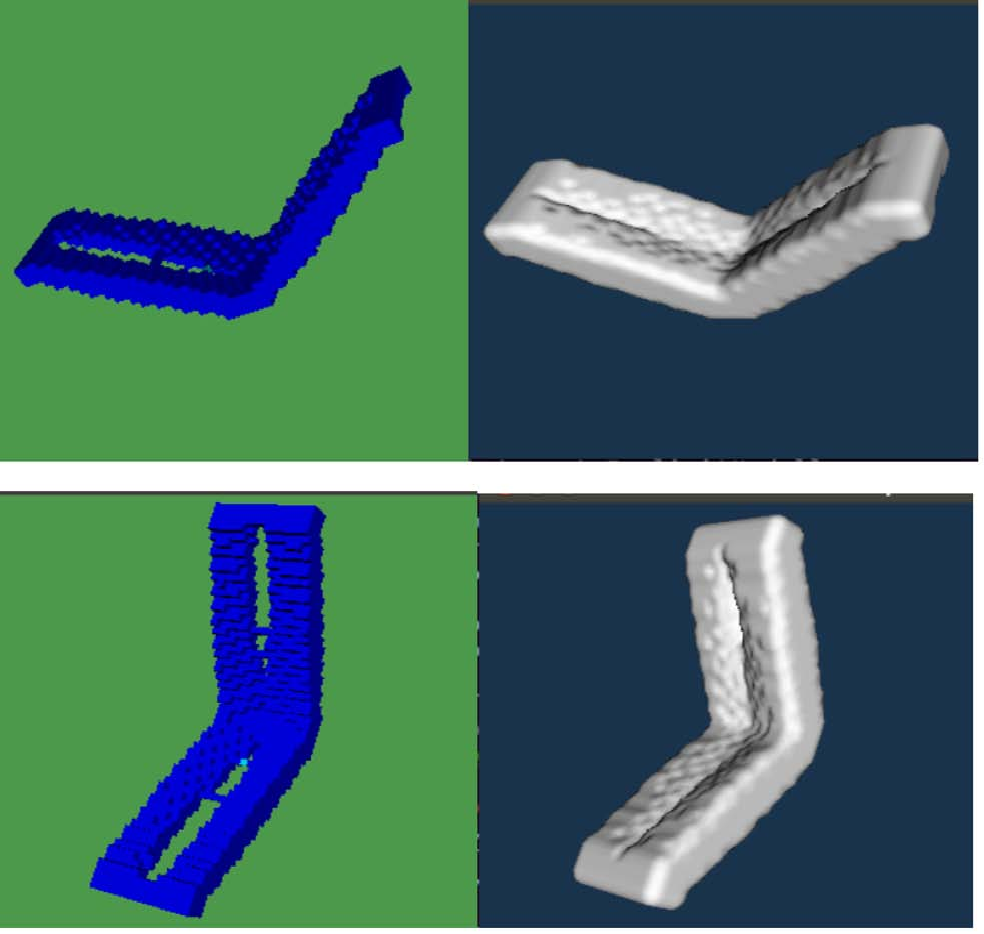
\includegraphics{Pictures/contouring.pdf}}\\
   \caption{Contour Filtering tool after Implicit Modelling}
\end{figure}

A further idea to solve this problem is to convert at the first step the volume data into point data
and only then present it to the Contour Filtering Tool. This will be implemented in the next
milestone.

The next step was to create a coarser mesh from the fine one. The triangles that represent the
isosurface can be reduced with the Decimation tool. A smoothing step is necessary in between
to get the new connections right. The top part of figure [2] shows a 50 \% reduction of the
triangles, a noticeable difference can not be perceived. On the lower part a 90 \% reduction is
obtained, it is nevertheless still difficult to see a difference. Triangle meshes can be easily
coarsened since there are many open source algorithms that simplify the triangles. VTK has the
decimation tool which works for 3D triangle data.

\begin{figure}
\centering
   \scalebox{0.4}{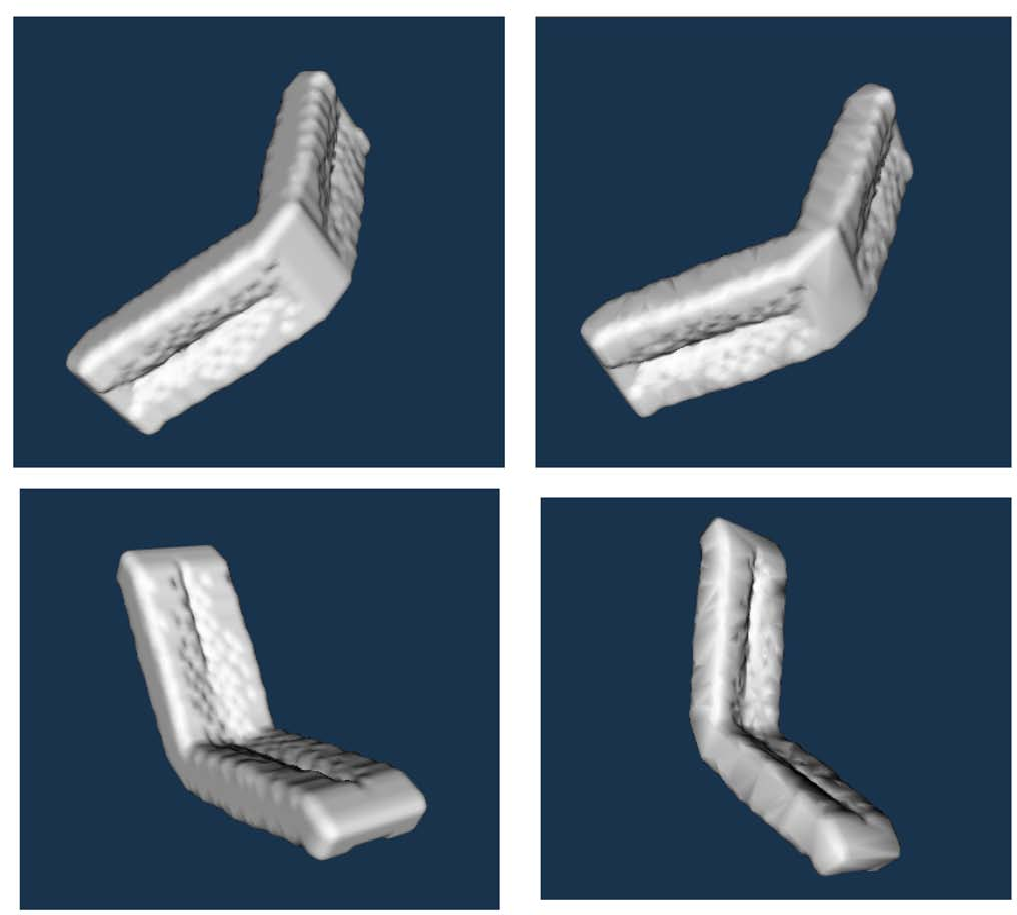
\includegraphics{Pictures/Decimation.pdf}}\\
   \caption{Decimation of triangles. \textit{Top:} 50\% \textit{Lower:}90\%}
\end{figure}

\subsection{The Long Road to NURBS}
There are two possible roads to go from the voxel data to the NURBS representation.
\subsubsection{Quad Contouring}
This approach uses the dual contouring algorithm as first step in order to obtain a quad mesh
representation from the voxel data. The first challenge is to implement correctly the algorithm
with the ideas presented in [1]. The original marching cubes algorithm is
implemented in VTK but the source code is not public, therefore not only an extension
of it is needed, but a full implementation. Once this first step is done, the quads will be chosen for the
NURBS parametrization. A second step considers multiple smaller quads which have to be
combined into one larger patch. This is another challenge, since the remeshing of quad meshes
is not as straight forward as with the triangles. Different approaches have been taken in order to
achieve this coarsening. In [2] an incremental and greedy approach, which is based on local operations only, is presented. It depicts an iterative process which performs local optimizing, coarsening and smoothing operations. Another approaches, like
the one presented in [3] uses smooth harmonic scalar fields to simplify the mesh.
%2= “Practical quad mesh simplification”
%3= “Harmonic Functions for Quadrilateral Remeshing of Arbitrary Manifolds”


\subsubsection{Multiresolution Analysis of Arbitrary Meshes}
With this approach there is no need to apply a Dual Contouring algorithm, since it takes as
beginning data the triangles from the Marching Cubes. The main concepts are shown in the paper
of the same name [4]. It mainly takes a series of intermediate steps which permits a parametrization of data. It includes a partitioning scheme based on the ideas of the Voronoi Diagrams and Delaunay triangulations. Large patches or quads are obtained with this method. Further discussion on this approach is explained in the following section.

%4=reference to MAAM, a.k.a Benni's favorite paper!

Both approaches have not been implemented in open source documentation, therefore it will be
a long road to achieve what is required. For the first part the second
road was chosen and in case it leads to a dead end, the first way will be taken into consideration.

%END JC